% Results
%
%	some important things to know
% 	experimental parts in the chapter results
%	numerical results or so-called data
%	order of presentation
% 	cross references

\chapter{Results}

\section{FFT}

\begin{figure}
\caption{Spectrogram of the beam position taken on the 16 October 2012}
\centering
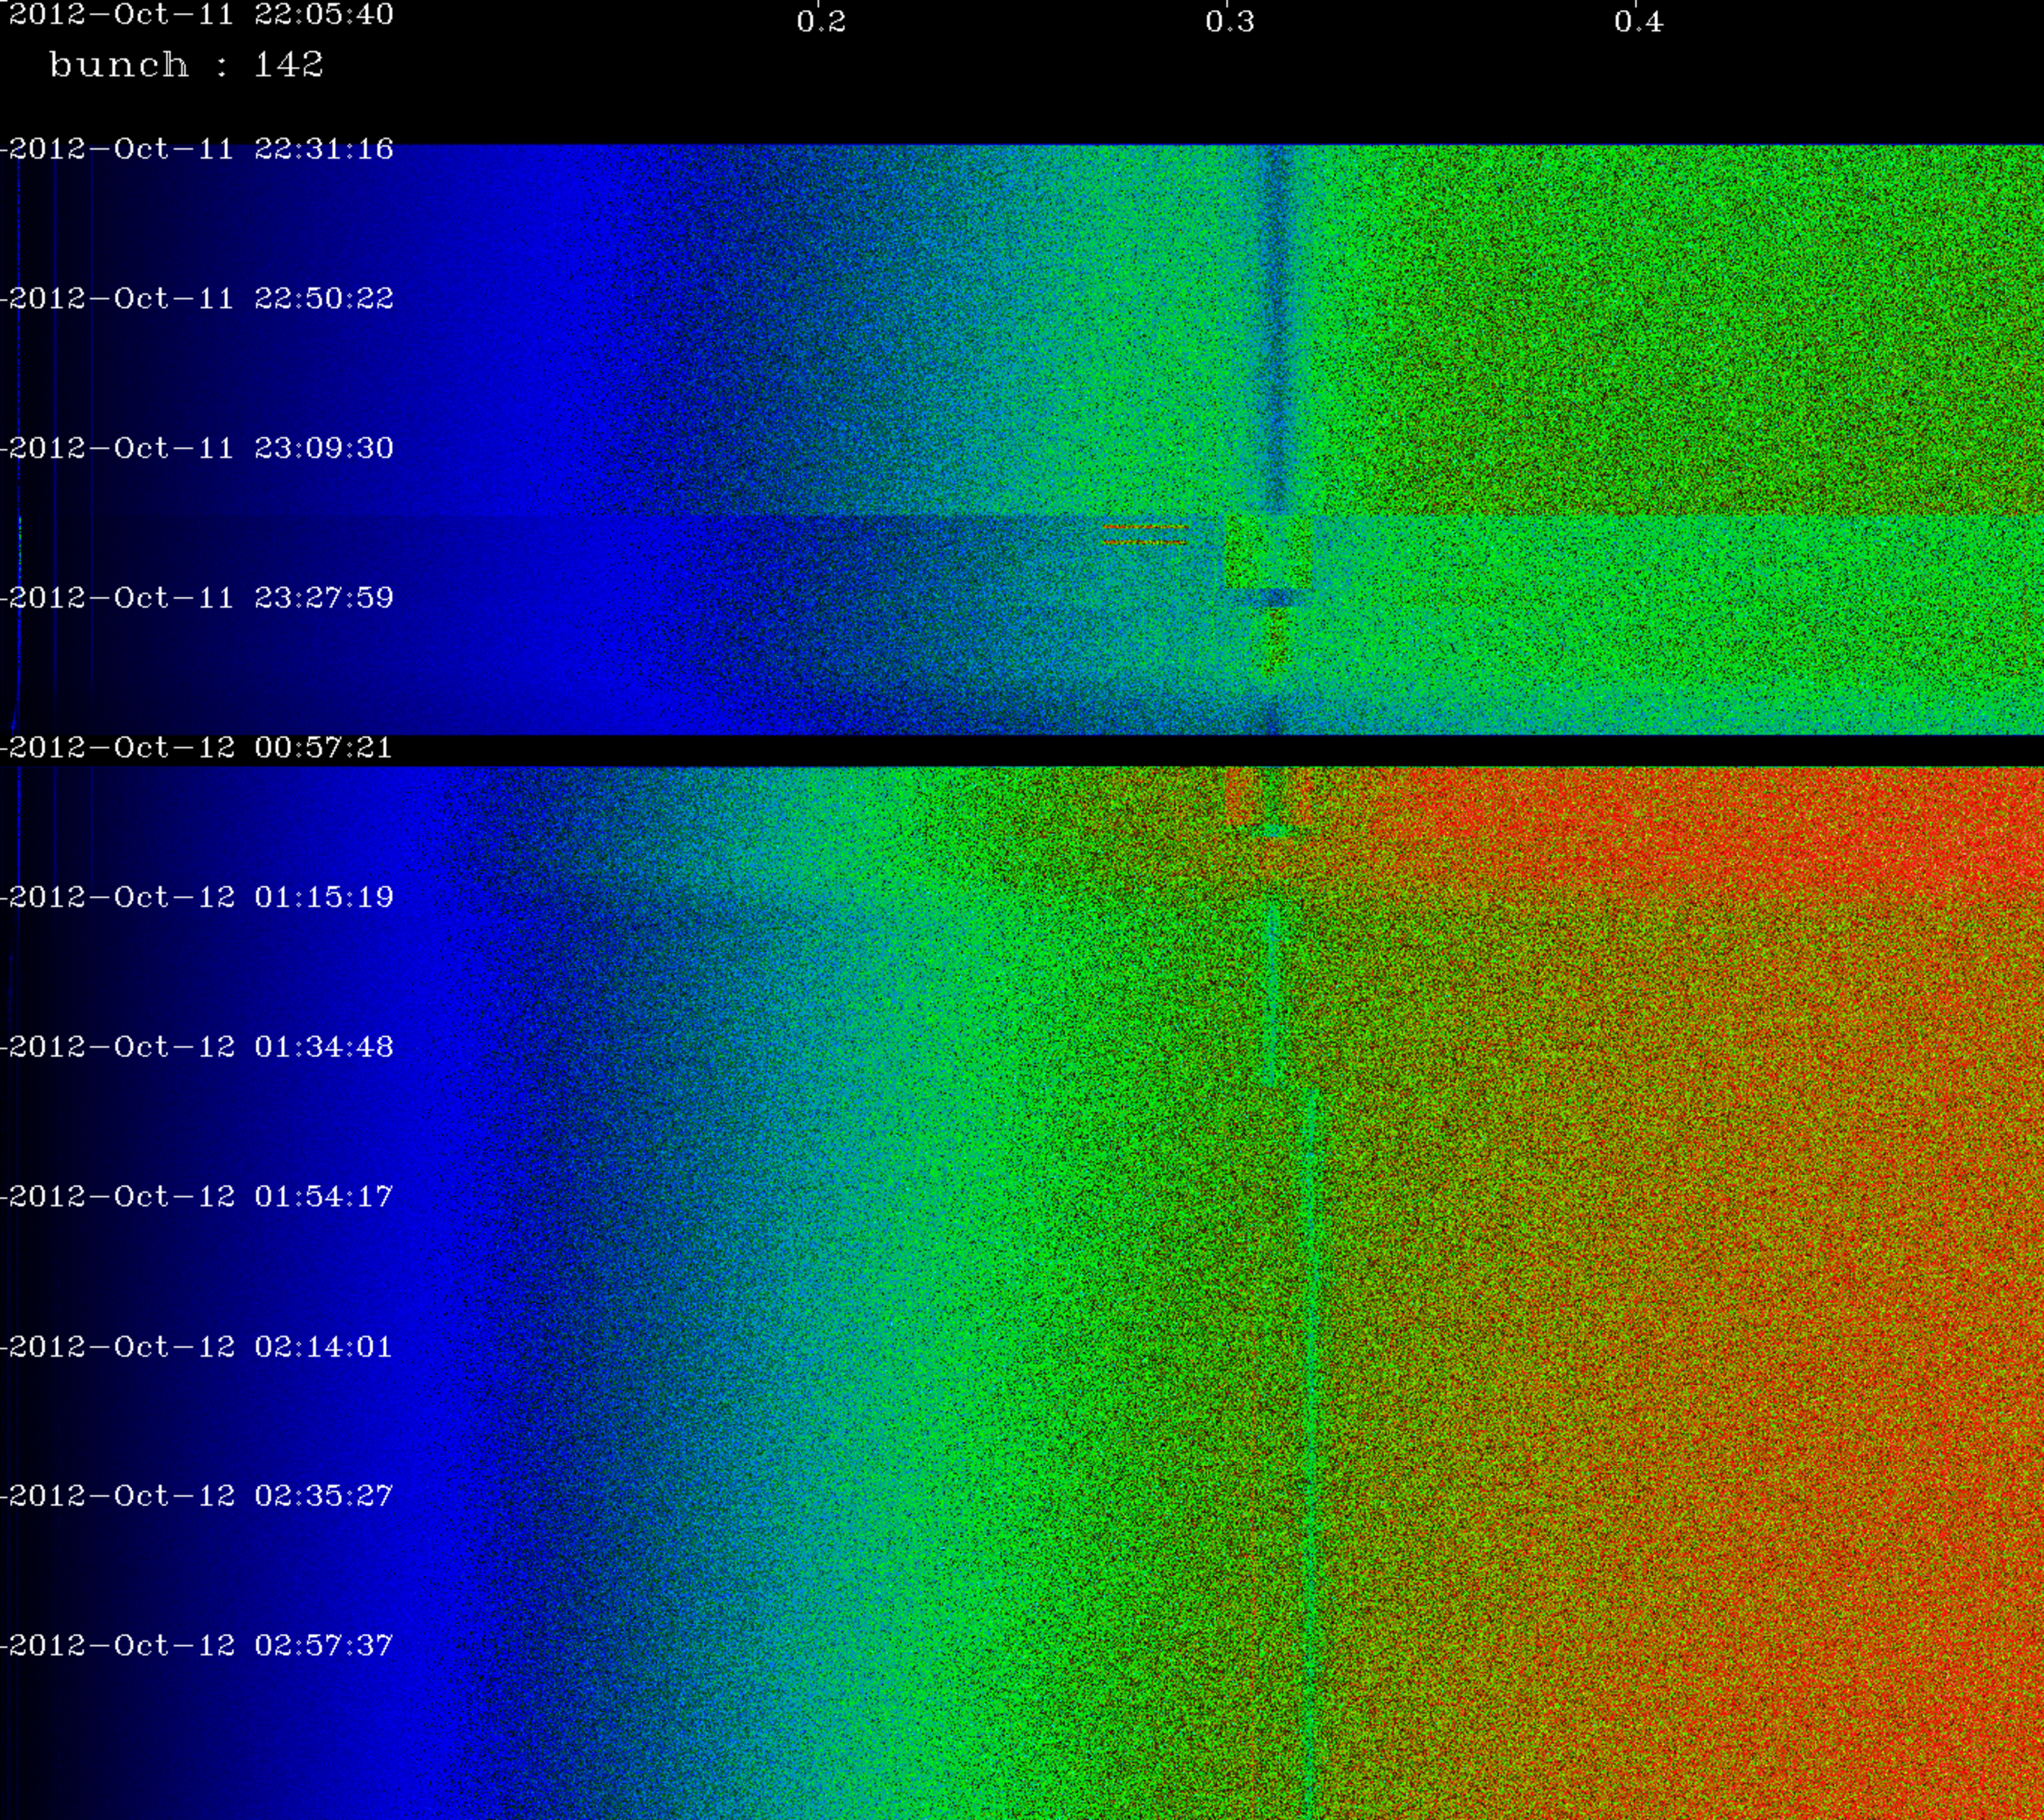
\includegraphics[scale=0.2]{spectrogram.pdf}
\end{figure}

\section{SVD}

\section{FFT uing GPU}

   \subsection{Performances}

\begin{figure}
\caption{Time flow with different implementations and with 3000 bunches of 
2048 points each.}
\centering
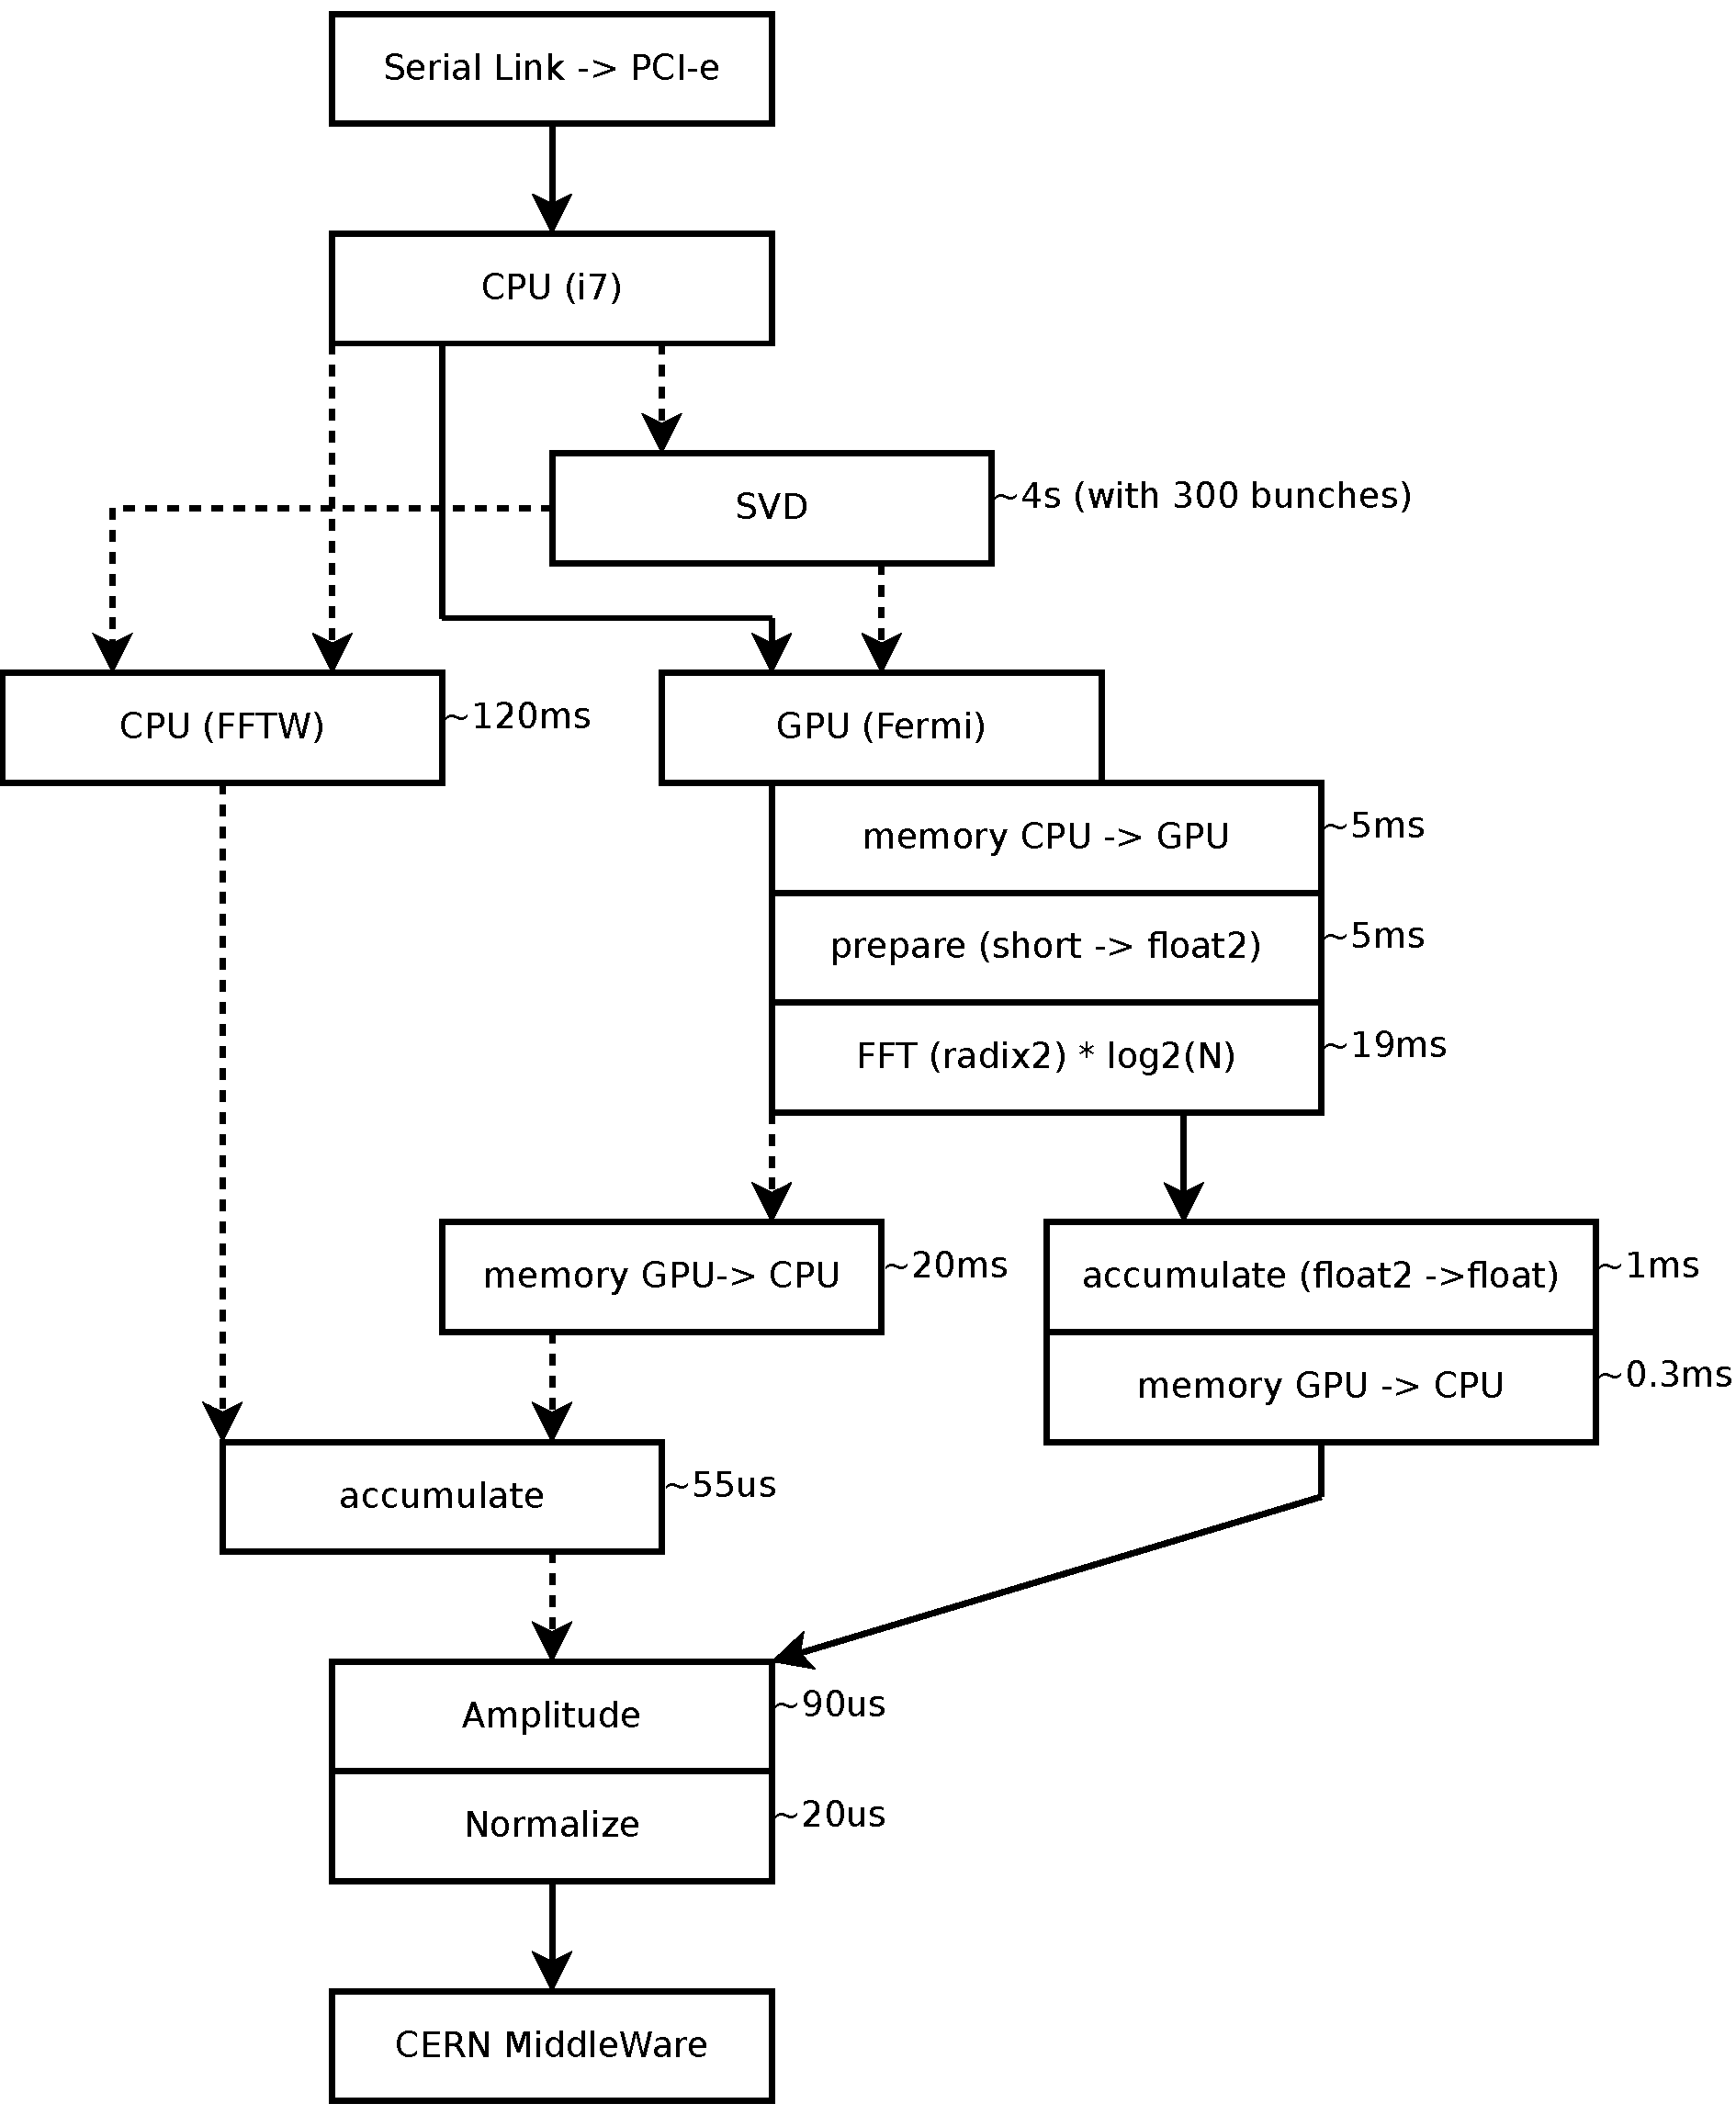
\includegraphics[scale=0.4]{PC-flow.pdf}
\end{figure}

   \subsection{Pipelining}

   Pipelining was tested and used in the process and it was possible to
   win around 15\% in performances around it.

   \subsection{Memory}

